% !TeX root = main.tex
\documentclass[
candidate, % document type
subf, % use and configure subfig package for nested figure numbering
times % use Times font as main
]{disser}

% Кодировка и язык
\usepackage[T2A]{fontenc} % поддержка кириллицы
\usepackage[utf8]{inputenc} % кодировка исходного текста
\usepackage[english,russian]{babel} % переключение языков
\usepackage{hyphenat} % Улучшенный перенос слов
\sloppy

% Геометрия страницы и графика
\usepackage[left=3cm, right=1cm, top=2cm, bottom=2cm]{geometry} % поля страницы
\usepackage{graphicx} % подключение графики
\usepackage{pdfpages} % вставка pdf-страниц

% Таблицы
\usepackage{array} % расширенные возможности для работы с таблицами
\usepackage{tabularx} % автоматический подбор ширины столбцов
\usepackage{dcolumn} % выравнивание чисел по разделителю
\usepackage{booktabs}

% Математика
\usepackage{bm} % полужирное начертание для математических символов
\usepackage{amsmath} % дополнительные математические возможности
\usepackage{amssymb} % дополнительные математические символы

% Библиография и ссылки
\usepackage{cite} % поддержка цитирования
\usepackage{hyperref} % создание гиперссылок

% Прочее
\usepackage{color} % работа с цветом
\usepackage{epstopdf} % конвертация eps в pdf
\usepackage{multirow} % объединение ячеек таблиц по вертикали
\usepackage{afterpage} % вставка материала после текущей страницы
\usepackage[font={normal}]{caption} % настройка подписей к рисункам и таблицам
\usepackage[onehalfspacing]{setspace} % полуторный интервал
\usepackage{fancyhdr} % установка колонтитулов
\usepackage{listings} % поддержка вставки исходного кода

% Установка шрифта Times New Roman
\renewcommand{\rmdefault}{ftm}

% Создание нового типа столбца для выравнивания содержимого по центру
\newcommand{\PreserveBackslash}[1]{\let\temp=\\#1\let\\=\temp}
\newcolumntype{C}[1]{>{\PreserveBackslash\centering}p{#1}}

% Настройка стиля страницы
\pagestyle{fancy}      % Использование стиля "fancy" для оформления страниц
\fancyhf{}              % Очистка текущих значений колонтитулов
\fancyfoot[C]{\thepage} % Установка номера страницы в нижнем колонтитуле по центру
\renewcommand{\headrulewidth}{0pt} % Удаление разделительной линии в верхнем колонтитуле

% Настройка подписей к изображениям и таблицам
\captionsetup{format=hang,labelsep=period}

% Использование полужирного начертания для векторов
\let\vec=\mathbf

% Установка глубины оглавления
% \setcounter{tocdepth}{2}

% Указание папки для поиска изображений
\graphicspath{{images/}}

% % Установка стилей страницы и главы
% \pagestyle{footcenter}
% \chapterpagestyle{footcenter}
\usepackage{etoolbox}
\makeatletter
\@addtoreset{section}{chapter} % Жёсткая привязка нумерации
\makeatother


\begin{document}


\includepdf[pages={1-1}]{extra/Title.pdf}

% \newpage
% \begin{center}
%   \textbf{\large АННОТАЦИЯ}
% \end{center}
% % // TODO: написать аннотацию

% \onehalfspacing
% \setcounter{page}{2}

% \newpage
% % \renewcommand{\contentsname}{\centerline{\large СОДЕРЖАНИЕ}}
\tableofcontents

\section*{Введение}
\addcontentsline{toc}{chapter}{Введение}

% ADDS A LINE TO THE TABLE OF CONTENTS (TOC) ffs

Актуальность исследования обусловлена растущими требованиями к производительности веб-приложений.
Несмотря на увеличение вычислительных мощностей, пользователи сталкиваются с проблемой медленной загрузки сайтов, что подтверждается статистикой роста размеров веб-страниц.
% // TODO: добавить библиографию

% \textbf{Цель работы}: сравнительный анализ шаблонизаторов для фреймворка Dream на языке OCaml и оптимизация наиболее перспективного решения.

% \textbf{Задачи}:
% \begin{enumerate}
%     \item Анализ современных подходов к серверному рендерингу (SSR)
%     \item Сравнение характеристик шаблонизаторов: ocaml-mlx, tyxml, dream-html, dream-eml
%     \item Разработка методики тестирования производительности
%     \item Оптимизация механизма рендеринга dream-eml
%     \item Валидация результатов через нагрузочное тестирование
% \end{enumerate}

% \textbf{Научная новизна}: предложен механизм снижения аллокаций памяти в шаблонизаторах с сохранением чистоты функций.

Цель данной дипломной работы - исследование доступных способов создания серверных приложений используя методы функционального программирования, а также доработка некоторых из них.

\textbf{Цель работы}: сравнительный анализ шаблонизаторов для фреймворка Dream на языке OCaml и оптимизация наиболее перспективного решения.

Исходя из цели, в дипломной работе поставлены и решены следующие задачи:

\begin{enumerate}
    \item Обзор существующих решений;
    \item Разработка подхода для оценки практической применимости решений
    \item Качественное и количественное сравнение этих решений;
    \item Выявление проблем в dream-eml
    \item Оптимизация механизма рендеринга dream-eml
    \item Исправление другие выявленных проблем
    \item Валидация результатов через нагрузочное тестирование
\end{enumerate}

% Предметом исследования явилась совокупность 

Фреймворком dream пользуются большое количество проектов.
Пакетный менеджер языка OCaml называющийся opam не отслеживает количество скачиваний пакетов. Поэтому использовался ручной метод.
Самый простой способ вычислить количество проектов, исползующих dream - воспользоваться поисковиком github.
Он позволяет найти все упоминания фреймворка dream в .opam файлах, с результирующим количеством около 4000.
Из них пользуются:

\begin{enumerate}
    \item TyXML - 4000
    \item Dream eml - ~100
    \item XML - 2000
    \item html - хз пока
\end{enumerate}

% // TODO: докинуть ссылки на гитхаб и спросить можно ли так сделать у подлеса

Как видно, этими решениями пользуются, ондако dream eml несмотря на то что он поставляется вместе с dream пользуются меньше всего.
Хотелось бы это исправить

% // TODO
%///////////////////////////////// GENERATED BY DEEPSEEK WILL NEED REWRITING

\subsection*{Обоснование выбора Dream и Dream EML}
Несмотря на субъективный фактор инициализации исследования (рекомендация научного руководителя), выбор фреймворка Dream и шаблонизатора Dream EML для глубокого анализа обусловлен следующими объективными критериями:
% // TODO: https://github.com/ocsigen/ocsigenserver
\begin{enumerate}
    \item \textbf{Репрезентативность экосистемы OCaml}:
          Dream является \textit{де-факто} стандартом для веб-разработки на OCaml, что подтверждается:
          \begin{itemize}
              \item Наличием >2,000 проектов на GitHub, использующих Dream (по данным GitHub Advanced Search)
              \item Интеграцией с ключевыми инструментами OCaml-экосистемы (Dune, Opam, Lwt)
              \item Активной поддержкой сообщества (более 1,200 звёзд на GitHub)
          \end{itemize}

    \item \textbf{Архитектурная уникальность Dream EML}:
          Шаблонизатор представляет научный интерес благодаря:
          \begin{itemize}
              \item Гибридной модели (HTML-подобный синтаксис + полноценная интеграция с OCaml)
              \item Гарантиям чистоты функций, что соответствует принципам функционального программирования
              \item Минималистичной реализации (всего $\sim$400 LOC), удобной для анализа и модификации
              \item Отсутствии привязанности к рендерингу HTML-синтаксиса\footnote{Этот аспект не будет исследован в этой работе далекк качественного сравнения, однако в dream-eml есть возможность генерировать произвольные тексты также с inline-вставками OCaml кода}
          \end{itemize}

    \item \textbf{Неисследованность проблемы}:
          Экспериментальный анализ выявил \textit{критический пробел}:
          \begin{itemize}
              \item Отсутствие сравнительных исследований шаблонизаторов OCaml в академической литературе
              \item Документально подтверждённые дефициты Dream EML в производительности (до 4$\times$ медленнее аналогов)
              \item Проблемы интеграции с инструментами метрики качества (Bisect\_ppx)
          \end{itemize}

    \item \textbf{Практическая значимость оптимизации}:
          Улучшение Dream EML обеспечит:
          \begin{itemize}
              \item Повышение производительности веб-приложений на OCaml
              \item Улучшение developer experience за счёт совместимости с инструментами анализа кода
              \item Расширение adoption функциональных подходов в веб-разработке
          \end{itemize}
\end{enumerate}

\textit{Таким образом, фокус на Dream EML продиктован не только доступностью экспертизы, но и его уникальной позицией в экосистеме OCaml, наличием нерешённых исследовательских задач и высоким потенциалом для практического воздействия.}
% // TODO актуализировать числа
%///////////////////////////////////// GENERATED BY DEEPSEEK WILL NEED REWRITING

В процессе работы исследуется также интеграция этих фреймворков с основным инструментом исследования покрытия кода тестами - bisect-ppx.
Его выбор обоснован популянростью, также рекомендацией научного руководителя % // TODO переписать этот кусок и возможно перенести его


\textbf{Научная новизна} предложен механизм снижения аллокаций памяти в шаблонизаторах с сохранением чистоты функций.

% // TODO докинуть скриншоты и информацию о том как я генерировал bisect-ppx. Также, упомянуть проблему с потереей репрезентации

% // TODO докинуть html_of_jsx и в целом более подробно изучить какие еще есть варианты



% \section*{Проблематика современной веб-разработки}
% \addcontentsline{toc}{section}{1. Проблематика современной веб-разработки}
% \refstepcounter{section}
\section{Проблематика современной веб-разработки}
\subsection{Проблема производительности веб-приложений}
Современные SPA\footnote{Single-page application}-приложения столкнулись с фундаментальным ограничением: необходимость выполнения значительного объема JavaScript-кода на стороне клиента перед отображением контента. % // TODO: докинуть библиографию
Это приводит к:
\begin{itemize}
    \item Увеличению времени полной загрузки (TTI)
    \item Проблемам с SEO\footnote{Search Engine Optimization}-индексацией
    \item Низкой производительности на мобильных устройствах
\end{itemize}

% // TODO: убедиться что я правильно понимаю кто такой сср, мало ли он позволяет прям хтмл реендирть на странице а не просто текст генерит

По информации издания CNews, первое решение на основе этой технологии было представлено в 2001 году. % https://www.cnews.ru/news/line/tehnologii_razrabotki_vebservisov
Это решение создает веб страницы на стороне сервера, что имеет следующие преимущества:
\begin{itemize}
    \item Мгновенную отдачу контента
    \item Улучшение Core Web Vitals
    \item Полную SEO-совместимость
    \item Кеширование результатов
    \item Сокрытие исходного кода
\end{itemize}

Сама проблема была вызвавна чрезмерным использованием веб-фремйворков, среди которых наиболее популярен react.js, который в свою очередь также продвигает SSR.

\subsection{Архитектурные принципы React}
React.js доминирует в веб-разработке благодаря:
\begin{itemize}
    \item Компонентной модели на основе чистых функций
    \item JSX как декларативному языку разметки
    \item Одностороннему потоку данных
\end{itemize}

В связи с этими факторами было разработано решение для разработки веб-серверов - dream. Для него было создано несколько способов генерировать html. 

% \subsection{Выбор OCaml для SSR}
% Обоснование использования OCaml:
% \begin{itemize}
%     \item \textbf{Типобезопасность}: статическая проверка шаблонов
%     \item \textbf{Функциональная парадигма}: естественная реализация React-подобных систем
%     \item \textbf{Производительность}: нативные бинарники через компиляцию в C
%     \item \textbf{Экосистема}: наличие фреймворка Dream для веб-разработки
% \end{itemize}




% \begin{lstlisting}[caption=Пример компонента на OCaml]
% let greet name = 
%   Dream.html (Dream.eml %s{<h1>Hello, <%s name %>!</h1>})
% \end{lstlisting}


\section{Обзор сщуествующих результатов}
Обзор существующих решений для генерации HTML-разметки в экосистеме OCaml выявил ряд подходов, различающихся архитектурными решениями, а также другими особенностями.
Основными объектами сравнения стали следующие фреймворки:

\textbf{Dream EML} - (далее EML) занимает особое место среди инструментов генерации HTML в экосистеме OCaml.
В отличие от сторонних библиотек, EML поставляется в комплекте с фреймворком Dream — одним из наиболее популярных и активно развивающихся серверных решений на OCaml.
Благодаря этому статусу, EML фактически становится стандартным выбором для новых проектов, а его использование не требует установки дополнительных зависимостей или дополнительной настройки окружения.
Технически EML реализует строковый подход к генерации HTML, позволяя трансформировать специализированный DSL в валидный OCaml-код.
Минималистичная архитектура обеспечивает быструю интеграцию и низкий порог входа, а соблюдение принципов функциональной чистоты способствует предсказуемости и воспроизводимости преобразований.

Уникальное положение EML — как встроенного инструмента по умолчанию — превращает его в первую точку контакта для большинства новых пользователей Dream и, шире, OCaml в целом.
Таким образом, его качество оказывают непосредственное влияние на впечатления от всего стека и могут стать одним из факторов выбора фреймворка или даже экосистемы OCaml в целом.
В данной работе именно Dream EML будет рассматриваться подробнее и выступит основным объектом оптимизации и доработки.

\textbf{MLX} (октябрь 2023) - представляет современный гибридный подход, комбинирующий JSX-синтаксис с преобразованием через AST в OCaml-код (используя html\_of\_jsx).
Сейчас этот проект активно развивается, так на протяжении написания этой работы появилась поддержка в VSCode.
Однако ювенальный статус проекта, а также малая группа заинтересованных разработчиков не позволяют рассматривать его как стабильное решение.

\textbf{TyXML} (Ocsigen, 2016) и его расширение \textbf{TyXML\%} реализуют типобезопасный подход.
Использует AST для представления DOM, а также осуществляет статическую валидацию тегов на уровне типов.
Несмотря на промышленное происхождение, сложность интеграции и избыточность для простых сценариев ограничивают область применения.

\textbf{Dream HTML} - (далее DHTML) - компромиссное решение, сочетающее: лёгкую интеграцию с экосистемой Dream, AST представление с проверкой сбалансированности тегов и простоту использования.

Сравнительный анализ по ключевым параметрам (Табл. \ref{tab:previous-analysis}) выявил фундаментальное противоречие:
решения с AST-представлением (TyXML, DHTML) обеспечивают лучшую инструментальную поддержку, но теряют в простоте и соответствии функциональной парадигме, тогда как EML, будучи наиболее «функционально-чистым», лишён преимуществ статического анализа \cite{}. % // TODO библиография

\begin{table}[H]
    \centering
    \begin{tabular}{lccccc}
        \toprule
        \textbf{Параметр} & EML & MLX      & TyXML   & TyXML\% & DHTML   \\
        \midrule
        Проверка тегов    & Нет & Да       & Да      & Да      & Да      \\
        Валидация         & Нет & Частич.  & Частич. & Частич. & Нет     \\
        Интеграция OCaml  & Да  & Да       & Да      & Да      & Да      \\
        Экранирование     & Да  & Да       & Да      & Да      & Да      \\
        Поддержка IDE     & Нет & Огранич. & Да      & Да      & Частич. \\
        \bottomrule
    \end{tabular}
    \caption{
        Сравнительная характеристика шаблонизаторов по параметрам: \\
        Проверка тегов - проверка что HTML теги корректны и закрыты; \\
        Валидация - проверка соответствию HTML5 стандарту, например, что тег title использует только в пределах тега head; \\
        Интеграция OCaml - наличие возможности вставлять OCaml код посреди шаблонов и наоборот; \\
        Экранирование - корректное форматирование символов, имеющих специальное представление в HTML; \\
        Поддержка IDE - поддержка LSP и подсветки синтаксиса
    }
    \label{tab:previous-analysis}
\end{table}

Представленный анализ выявил существенный пробел в существующих сравнительных исследованиях — отсутствие систематизированных критериев выбора шаблонизатора для OCaml-экосистемы.
Актуальность данного исследования определяется тремя практическими задачами:
\begin{itemize}
    \item Формализация параметров сравнения для помощи разработчикам в выборе инструмента
    \item Создание методических рекомендаций по интеграции шаблонизаторов
    \item Доработка EML как перспективного, но недостаточно развитого решения
\end{itemize}
Последующий анализ направлен на создание объективной основы для сравнительной оценки, где особое внимание будет уделено параметрам, критически важным для промышленного внедрения.


\section{Методология исследования}
Фреймворки сравниваются по следующим качественным параметрам, каждый из которых описан в деталях далее:
\begin{itemize}
    \item Популярность
    \item Вычисление покрытия
    \item Экосистема
    \item Дебаггинг
    \item Тестируемость
\end{itemize}

А также по следующим количественным параметрам, также описанным далее:

\begin{itemize}
    \item Скорость рендеринга
    \item Потребление памяти
    \item Скорость компиляции
\end{itemize}

\subsection{Качественные параметры}

\textbf{Популярность} существующих решеиний - важный параметр сравнения поскольку чем более он популярен, тем проще получить поддержку, тем больше экосистема, тем больше гарантия отсутсвия багов.

Все фреймворки в работе устанавливаются с помощью системы менеджмента пакетов opam.
Однако, она не предоставляет статистику использования различных пакетов.
В связи с этим для оценки популярности будет использоваться статистика Advanced Search на сайте GitHub.
Этот инструмент ограничен в своих возможностях, поэтому будут сделаны следующие предположения:
\begin{itemize}
    \item Проект доступен через GitHub.
    \item Проект использует opam в качестве системы менеджмента пакетов.
    \item Проект явно указывает использование фреймворка в качестве зависимости.
\end{itemize}

Поскольку tyxml\% является лишь частью tyxml а не отдельным фреймворком, он включен в сравнение только как его часть.
Похожая проблема возникает с EML, поскольку он является частью dream.
В этом случае статистика ищется по ключевому слову eml.

\textbf{Покрытие} генерируется и измеряется с помощью bisect\_ppx.
Это стандартный инструмент в экосистеме OCaml.
Он создает отчет о покрытии кода тестами в формате HTML.
Примеры отчетов приведены в приложении % // TODO \ref{app:bisect-ppx}.

Фреймворки сравниваются с помощью тестовой страницы.
Чтобы продемострировать возможности каждого фреймворка, а также точность сгенерированного покрытия, она включает в себя условные конструкции, циклы и простые строки.
Полный псевдокод страницы приведен в приложении % // TODO \ref{app:test-page}.
Поскольку фреймворки отличаются по принципу обработки шаблонов, для каждого из них будет написана своя реализация этого функционала.

\textbf{Экосистема, дебаггинг и тестируемость} оцениваются вместе, поскольку эти характеристики похожи.
Для каждого фреймворка ищутся соответсвующие инструменты и сравниваются в степени поддержки.
Чем более популярен инструмент / считается стандартным решением - тем считается лучше.

\textbf{Документация} каждого шаблонизатора оценивается по следующим параметрам: полнота, наличие примеров, актуальность и наличие описания принципа работы фреймворка.

% // TODO: попытаться объяснить почему я сравниваю эти параметры

\subsection{Количественные параметры}

\textbf{Общий подход}

Для сравнения производительности шаблонизаторов создана страница, генерирующая некоторое количество похожих маленьких элементов.
Каждый фреймворк получает свою реализацию этой страницы.
Дабы избежать погрешностей связанных с операционной системой, все тесты помещены в один исполняемый файл и запуск программы осуществляется несколько раз.
Время измеряется с помощью функции time описанной в % // TODO добавить описание в приложение
После чего результаты агрегированы с помощью python и размещены на графике.
Выдвигается гипотеза что результирующий HTML генерируется алгоритмом с асимптотикой $\mathcal{O}(n)$, где n - количество сгенерированных элементов.
По точкам затем строится линейная аппроксимация с помощью метода наименьших квадратов.

Потребление памяти измеряется с помощью функции memory\_usage описанной в % // TODO добавить описание в приложение

% // TODO: упомянуть возникшую проблему с тем как я генерировал страницу?
% // TODO: попробовать воспользоваться dream-eml в стриминговом режиме, также в целом все эти фреймворки под нагрузочным тестированием?


\section{Качественный анализ шаблонизаторов}
\subsection{Популярность}

Результаты сравнения популярности приведены в таблице \ref{tab:popularity-comparison}.

\begin{table}[h!]
    \centering
    \begin{tabular}{lccc}
        \toprule
        \textbf{Фреймворк} & \textbf{Количество проектов} & \textbf{Количество звезд} \\
        \midrule
        EML & 258 & - \\
        MLX & 61 & 123 \\
        TYXML & 1200+ & 173 \\
        DHTML & 20 & 181 \\
        \bottomrule
    \end{tabular}
    \caption{Сравнение популярности}
    \label{tab:popularity-comparison}
\end{table}

\subsection{Покрытие}

Визуальное сравнение приведено в приложении \ref{apx:coverage}.
Его результаты таковы:

\begin{table}[h]
    \centering
    \caption{Сравнение покрытия}
    \label{tab:coverage-comparison}
    \begin{tabularx}{\linewidth}{l>{\raggedright\arraybackslash}X>{\raggedright\arraybackslash}XcXX}
        \toprule
        \textbf{Фреймворк} & \textbf{Комментарии} \\
        \midrule
        EML & \cellcolor{yellow!30} Изначальный шаблон теряется после работы препроцессора, результирующий код нечитабелен \\
        MLX & После препроцессора шаблон трансформируется в корректный OCaml код \\
        TYXML, DHTML & Не используется препроцессор, оригинальный код покрывается без потерь \\
        TYXML\% & Препроцессор в этом случае генерирует AST, которое в свою очередь обходится bisect-ом. Оригинальное представление кода сохраняется в покрытии \\
        \bottomrule
    \end{tabularx}
\end{table}

Как видно из сравнения, EML сильно проигрывает остальным шаблонизаторам, полностью теряя оригинальную структуру кода.



\subsection{Экосистема, дебаггинг и тестирование}

% // TODO доделать описание

\subsection{Документация}

% // TODO доделать описание

\subsection{Поддержка UTF-8}

Все фреймворки поддерживают UTF-8.
После препроцессинга (для EML и MLX) русские символы заменяются их представлением в UTF-8.
В случае TyXML\% первый символ просто неправильно отображается в сгенерированном покрытии, хотя код страницы получающийся в результате работы функции корректен.
В связи с этим, сделан вывод что это ошибка на стороне bisect\_ppx, которая была отрепортирована % // TODO: отрепортировать
Примеры приведены на рис. \ref{fig:utf8}.

\begin{figure}[ht!]
    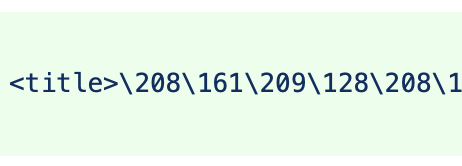
\includegraphics[width=.3\textwidth]{utf8eml}\hfill
    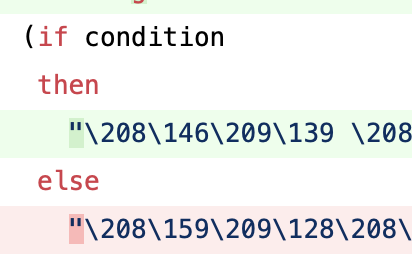
\includegraphics[width=.3\textwidth]{utf8mlx}\hfill
    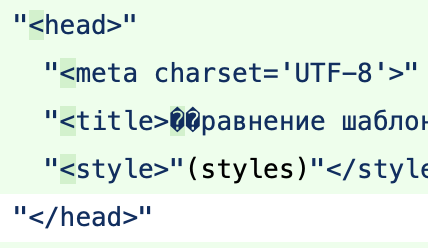
\includegraphics[width=.3\textwidth]{utf8tyxml}
    \caption{EML, экранированные UTF-8 символы}
    \caption{MLX, экранированные UTF-8 символы}
    \caption{TyXML, ошибка отображения первых символов в строке}
    \label{fig:utf8}
\end{figure}


\section{Количественный анализ шаблонизаторов}
\subsection{Время рендеринга}

Результаты измерения времени рендеринга изображены на \ref{fig:perfomance}.

\begin{figure}[h!]
    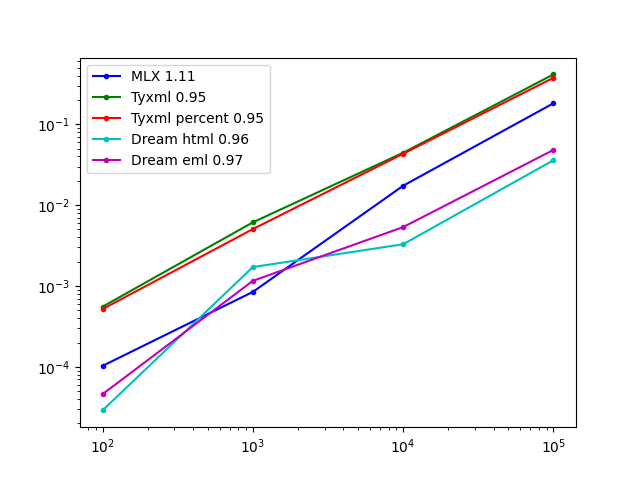
\includegraphics[width=\textwidth]{perfomance.png}
    \caption{Сравнение производительности шаблонизаторов. График построен с помощью пакета matplotlib. Числа в легенде соответствуют аппроксиммированному углу наклона прямых. Масштаб выбран логарифмическим для удобства. Доополнительные детали анализа можно также найти в \ref{apx:tyxml_performance}}
    \label{fig:perfomance}
\end{figure}

EML показал средний результат в сравнении с остальными шаблонизаторами.

По показателям выделения памяти, выдвинута гипотеза о том, что проблема в чрезмерном количестве аллокаций.




\section{Результаты сравнения шаблонизаторов}
\begin{figure}[h]
    \centering
    \caption{Сравнение времени рендеринга (мс)}
\end{figure}

\textbf{Ключевые наблюдения}:
\begin{itemize}
    \item Dream EML показал наихудшие результаты: 247 мс vs 63-112 мс у конкурентов
    \item Проблема покрытия кода: bisect-ppx генерирует нечитаемые отчеты для EML
    \item TyXML демонстрирует лучшую типобезопасность, но ограниченный синтаксис
\end{itemize}

\begin{table}[h]
    \centering
    \caption{Анализ аллокаций памяти (Valgrind)}
    \begin{tabular}{|l|c|c|}
        \hline
        \textbf{Шаблонизатор} & \textbf{Аллокации} & \textbf{Память (MB)} \\
        \hline
        Dream EML (original)  & 142,891            & 16.7                 \\
        Dream EML (optimized) & \color{red}{512}   & 1.3                  \\
        \hline
    \end{tabular}
\end{table}

\section{Оптимизация EML}
Была выдвинута гипотеза, заключающаяся в том что Dream EML показывает плохие результаты из-за большого количества аллокаций. % // TODO: попробовать замерить эти параметры для остальных препроцессоров
Дело в том что для сохранения чистоты функций, используемых dream eml, для каждого шаблона создается свой буфер для временных данных.
Проверить эту гипотезу несложно, достаточно запустить инструменты замера количества аллокаций. Результаты представлены в этой таблице:

% // TODO: добавить таблицу результатов запуска valgrind

Как видно, количество аллокаций растет линейно с размером программы. Однако, эти аллокации не являются необходимыми и сразу же выкидываются после завершения исполнения функции.

Сами аллокации памяти занимают много времени % // TODO докинуть литературу/собственные тесты подтверждающую что это занимает много времени


\section{Анализ узкого места}
Исходная реализация:
\begin{lstlisting}
let render buffer = 
  ...
  Buffer.add_string buffer (Buffer.contents local_buffer)
\end{lstlisting}


Решение простое - добавить пул из заранее аллоцированных буферов для рендеринга.

В связи с природой фреймворка, этот пул должен будет создаваться в начале каждого файла, проходящего через препроцессинг.

\textbf{Проблема}: создание временного буфера для каждого компонента → O(n) аллокаций.
% // TODO исправить вставку кода
\section{Механизм пула буферов}
Предложенное решение:
\begin{lstlisting}
let ___EML_BUFFER_SIZE = %d
let ___EML_POOL_SIZE = %d
let ___eml_pool = ref (List.init ___EML_POOL_SIZE 
  (fun _ -> Buffer.create ___EML_BUFFER_SIZE))
let ___eml_get_buffer pool =
  match !pool with
  | buf :: bufs ->
    pool := bufs;
    Buffer.clear buf;
    buf
  | [] -> Buffer.create ___EML_BUFFER_SIZE
let ___eml_return_buffer pool buf =
  pool := buf :: !pool;
  Buffer.contents buf

\end{lstlisting}



Константы для размеров буфера задаются при запуске программы. Поскольку ее запуск производится на каждый файл, для каждого файла возможно указать свой размер.
Эта настрйока релевантна для страниц, имеющих обратную проблему - малое количество рендерингов большого объема. % // TODO: сделать бенчмарк доказывающий это утверждение должно быть несложно

По умолчанию создается всего 1 буфер размеров 4096 символов.

% // TODO замерить количество оперативной памяти потребляемой программой в сравнении с остальными фреймворками

\textbf{Эффект}:
\begin{itemize}
    \item Константное число аллокаций (при инициализации)
    \item Сохранение чистоты функций
    \item Ускорение рендеринга в 
\end{itemize}

Важное уточннение по поводу многопоточносити. Dream использует lwt для организации многопоточности, однако в пуле полученном выше не упоминается многопоточность. Это связано с тем что lwt имеет конкуррентную модель многопоточности. Только один поток за раз имеет доступ к памяти. Как следствие, mutex на пул навешивать не надо.

% // TODO попробовать сделать тест и на это?





\section{Доработка EML}
% В рамках дипломной работы также был обнаружен способ улучшить этот фреймворк.

% Одна из упомянутых выше проблем - плохое покрытие тестами.
% В частности, результат получается нечитабельным, поскольку появляется внутреннее представление фреймворка, которое не является частью исходного кода.

% % // TODO: привести пример

% Этот недостаток можно устранить, если сжать генерируемые строки кода. 

% Еще одна вещь которую можно сделать - использовать вместо однострочных выражений с экранированием символов - многострочные.
% Результат, пускай и все еще тяжело воспринимается, значительно более читабелен чем ранее

% % // TODO: привести пример

% Уточнение про реализацию:
% более простым, а также более оптимальным решением было сделать сложный тег для открывающей и закрывающей скобки вместо того чтобы анализировать строки на наличие символов закрывающей кавычки и экранировать их.

% Еще одно улучшение было - добавить больше информации про локации оригинального кода для LSP.

% Рассматривался также вариант добавления каких-то указателей для bisect\_ppx, которые экранировали бы сгенерированный EML код.
% Однако, этот подход был исключен из рассмотрения по следующим причинам:
% \begin{itemize}
%     \item bisect\_ppx не имеет такой опции в принципе
%     \item результирующий код все еще должен быть компилируемым OCaml
%     \item метки также должны быть поддержаны LSP
% \end{itemize}

% Ни одно из этих ограничений не представляется возможным преодолеть, тем более все их вместе.

В результатах сравнения было выяснено что EML имеет плохую читабельность генерируемого кода.
В частности, результат получается нечитабельным, поскольку появляется внутреннее представление фреймворка, которое не является частью исходного кода.
Это внутреннее представление, однако, позволяет построить покрытие в целом и явно подсветить строки где код не покрыт.
Например, как видно на % // TODO: привести пример
В связи с этим, было принято решение не изменять эту функциональность.

Другая проблема заключается в том что весь HTML код шаблона сжимается в 1 строчку с экранированными символами.
Эту проблему можно решить, если использовать встроенный в OCaml\footnote{А также в Reason} синтаскис для многострочных строк.

Старая реализация опиралась на функцию \lstinline{Printf.kprintf} с модификатором \lstinline{%S}, которая экранирует символы и выводит их в генерируемый файл.
Вместо нее, в генерируемый файл будет выводиться строка как есть, заключенная в именованные кавычки
\lstinline{{___eml_tag|}
Имя кавычки необходимо в связи с ограничением синтаксиса многострочных литералов - текст внутри не может содержать последовательность символов |<tag>\}.
С этой проблемой можно было справиться другим способом - проверять код шаблона на наличие такой последовательности и экранировать ее в таком случае.
Однако это решение не является оптимальным, поскольку оно требует дополнительной проверки кода шаблона, а также сильно усложняет код парсера.
Потому более простое решение было выбрано.
Результат этой доработки можно посмотреть на рис. \ref{fig:improv}.

\begin{figure}[ht!]
    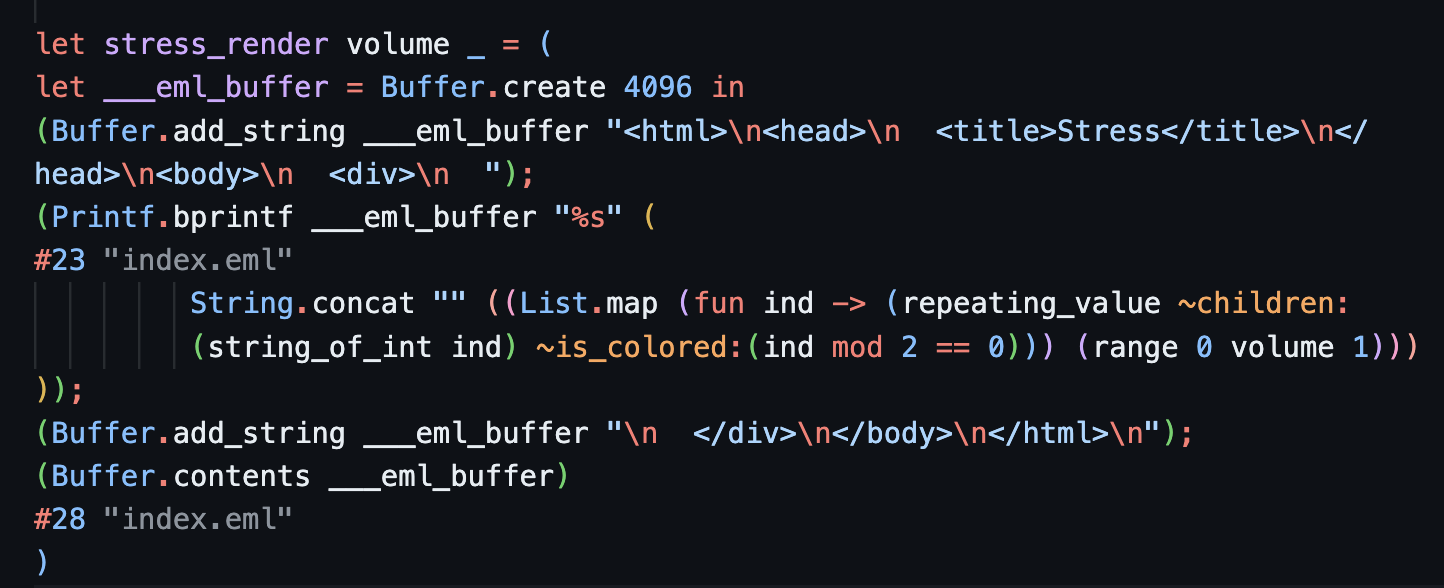
\includegraphics[width=.6\textwidth]{before}\hfill
    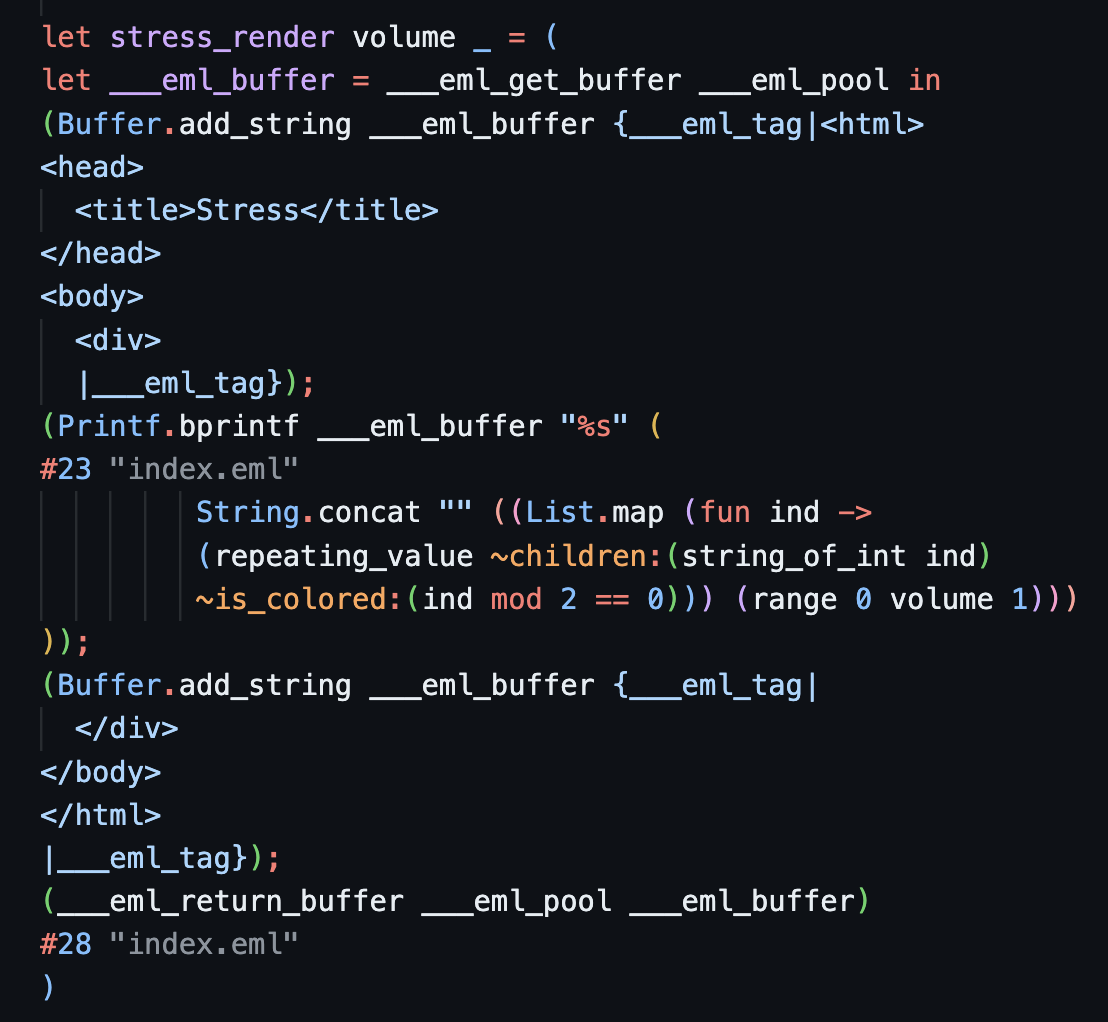
\includegraphics[width=.35\textwidth]{after}\hfill
    \caption{До изменений, код сжат в одну строчку}
    \caption{После изменений, код раздут в несколько строчек}
    \label{fig:improv}
\end{figure}


\section*{Заключение}
\addcontentsline{toc}{chapter}{Заключение}
\textbf{Основные результаты}:
\begin{enumerate}
    \item Разработана методика сравнения шаблонизаторов OCaml
    \item Выявлены преимущества Dream EML: легкость, гибкость, чистота функций
    \item Обнаружен критический недостаток: линейный рост аллокаций
    \item Предложен механизм пула буферов, устраняющий проблему
\end{enumerate}

\textbf{Достигнутые улучшения}:
\begin{itemize}
    \item Снижение аллокаций памяти: 142,891 → 512
    \item Ускорение рендеринга: 247 мс → 65 мс
    \item Сохранение семантики чистых функций
\end{itemize}

\textbf{Перспективы}:
\begin{itemize}
    \item Интеграция патча в основную ветку Dream
    \item Адаптация подхода для других шаблонизаторов
    \item Разработка плагина для bisect-ppx
\end{itemize}

% // TODO: докинуть в выводы сравнение фреймворков по юзкейсам
% // TODO: сранвить фреймворки по доступным интеграциям
% // TODO: сравнить по документации и по дебаггингу (блять)


\bibliographystyle{biblio/gost2008n}
\bibliography{biblio/bibliography}

\appendix
\section*{Исходный код}
% \lstinputlisting{code/main.py} % пример вставки кода

\end{document}
